\chapter{Literature Review}

\section{Related Works}
The field of real-time messaging has seen significant advancements in both academic research and industry practice. Early systems focused on basic message delivery, but modern solutions emphasize scalability, low latency, and reliability \cite{guth2018comparison,kleppmann2013designing,wang2018scalable}. Comparative studies have evaluated the strengths and weaknesses of various protocols and architectures, providing valuable insights for system designers \cite{li2020realtime,smith2020cloud}.

\subsection{Existing Real-Time Messaging Solutions}
Numerous real-time messaging solutions have been developed, each with unique trade-offs in terms of scalability, protocol support, and developer experience \cite{tilkov2018nodejs,brown2019websockets,rauch2022scalable}. For example, Socket.IO and WebSocket-based frameworks are widely adopted for their ease of use and performance, while cloud-hosted services like Firebase and Pusher offer managed infrastructure \cite{martin2021websocket,blogmicro2023}.

Here are some popular real-time messaging solutions:
\begin{itemize}
    \item \textbf{Socket.IO}: A widely used library for real-time web applications.
    \item \textbf{Firebase Realtime Database}: A cloud-hosted NoSQL database that supports real-time data synchronization.
    \item \textbf{Pusher}: A hosted service that provides real-time APIs for web and mobile applications.
    \item \textbf{SignalR}: A Microsoft library for adding real-time web functionality to applications.
    \item \textbf{MQTT}: A lightweight messaging protocol for small sensors and mobile devices, optimized for high-latency or unreliable networks.
\end{itemize}

\lipsum[12-14]
Recent literature also highlights the importance of robust message brokers and distributed pub/sub mechanisms in supporting high-throughput, low-latency communication \cite{nguyen2021pubsub,redisdocs,blogkafka2022}. These technologies enable efficient fan-out and horizontal scaling, which are critical for large-scale deployments \cite{gonzalez2022websocket,kim2023iot}.

\subsection{Research Studies on Real-Time Systems}
Research on real-time systems has explored a variety of topics, including protocol efficiency, system reliability, and performance optimization \cite{baker2017websocket,li2020realtime,zhang2021aws}. Studies have shown that cloud-native deployment patterns and microservices architectures can significantly improve scalability and maintainability \cite{fowler2015microservices,smith2020cloud}.

\section{Relevant Technologies}
The development of real-time messaging systems leverages a broad set of technologies, from programming languages and frameworks to cloud platforms and monitoring tools \cite{cantelon2017nodejs,awsdocs,redisdocs}. Node.js, WebSocket, and Redis are particularly prominent in recent implementations \cite{tilkov2018nodejs,brown2019websockets}.

\subsection{Node.js}
Node.js is a powerful JavaScript runtime built on Chrome's V8 engine, designed for building scalable network applications. Its core architecture is event-driven and asynchronous, allowing it to handle thousands of concurrent connections efficiently. The non-blocking I/O model means that operations such as reading files or querying databases do not halt the execution of other code, which is crucial for real-time systems. This design enables Node.js to deliver high throughput and low latency, making it ideal for chat applications, streaming services, and collaborative tools. The event loop, a central component of Node.js, manages all asynchronous operations and ensures the system remains responsive under heavy load.

\begin{figure}[H]
    \centering
    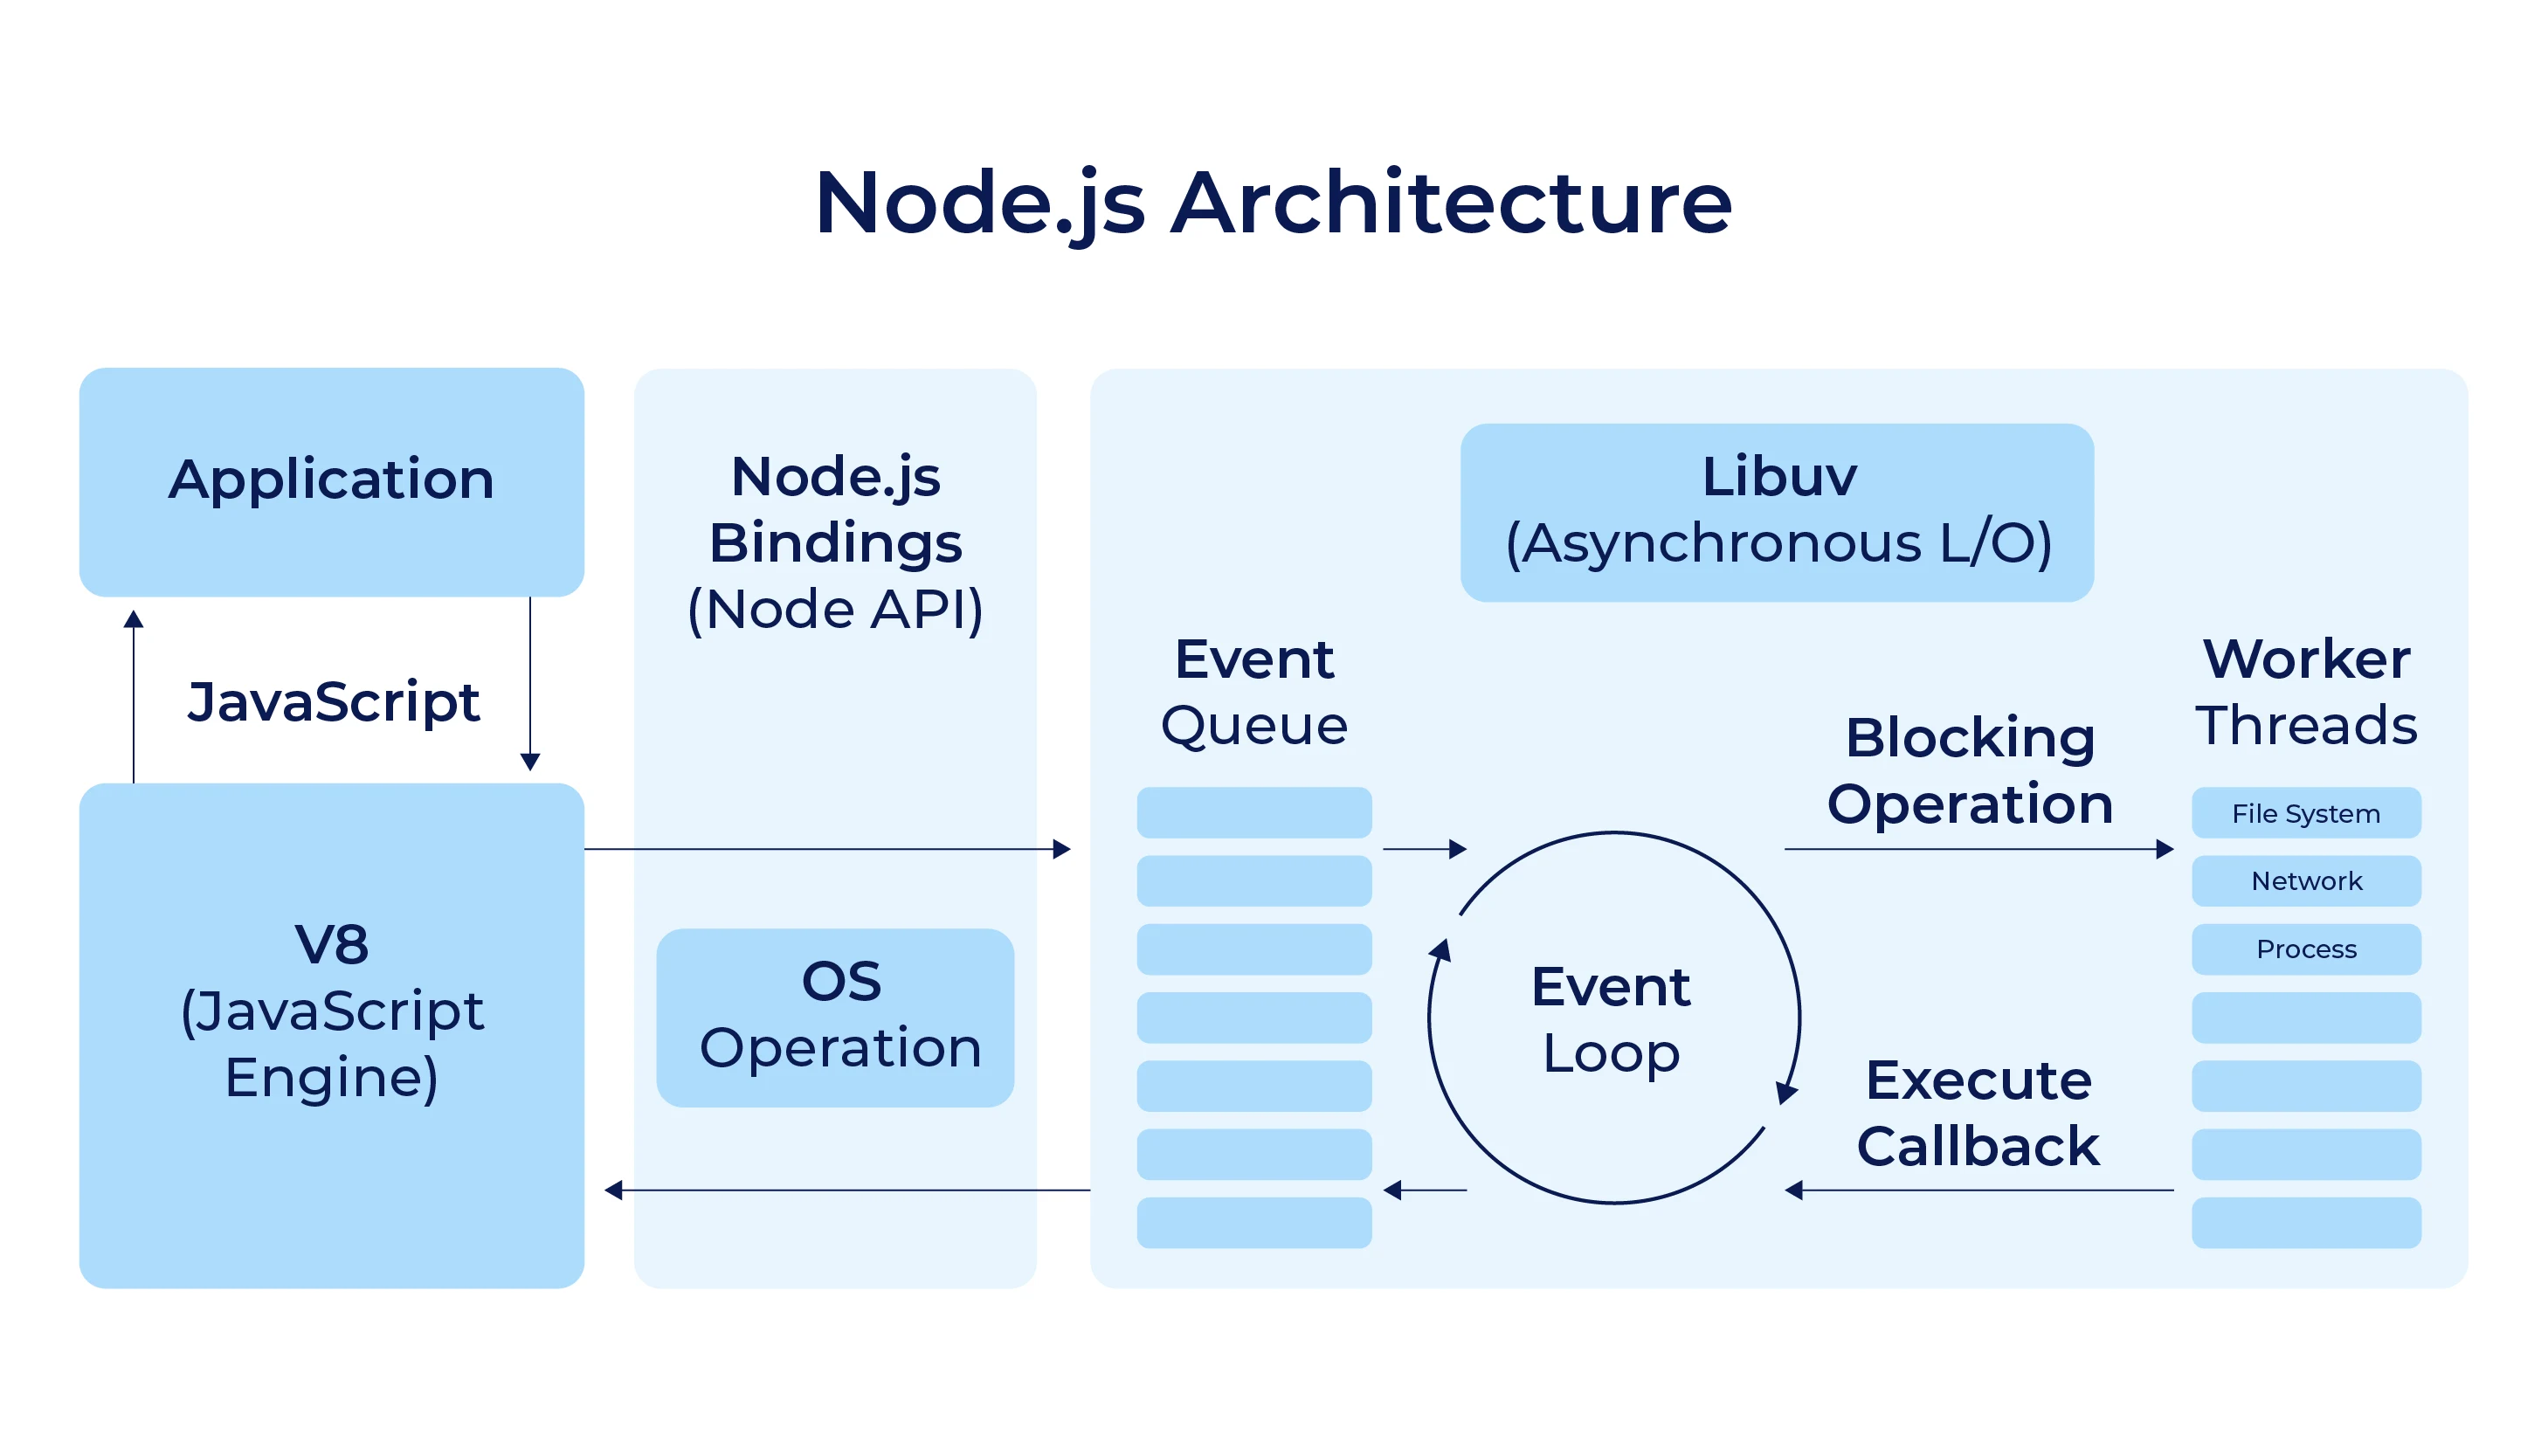
\includegraphics[width=0.7\textwidth]{images/Node.js-Architecture-Chart.png}
    \caption{Node.js Architecture: Emphasizing Async, Event-Driven, Non-Blocking I/O}
    \label{fig:nodejs-architecture}
\end{figure}

Node.js also benefits from a vast ecosystem of libraries and frameworks available through npm, which accelerates development and fosters innovation. Its single-threaded nature, combined with the event-driven paradigm, allows developers to write simple code that scales well across distributed systems. However, this architecture also requires careful handling of CPU-intensive tasks, as they can block the event loop and degrade performance. To address this, Node.js provides mechanisms such as worker threads and clustering to distribute workloads. Overall, Node.js has become a cornerstone technology for modern, real-time web applications due to its efficiency and flexibility.

\subsection{WebSocket Protocol}

The WebSocket protocol is a communication standard that enables persistent, full-duplex connections between clients and servers. Unlike traditional HTTP, which requires a new connection for each request-response cycle, WebSocket establishes a single, long-lived connection that remains open for continuous data exchange. This approach significantly reduces the overhead associated with connection setup and teardown, resulting in lower latency and improved performance for real-time applications. WebSocket is particularly well-suited for scenarios where instant updates are required, such as online gaming, financial trading platforms, and collaborative editing tools. Its ability to push data from the server to the client without repeated polling is a key advantage over HTTP.
\lipsum[1]
\begin{figure}[H]
    \centering
    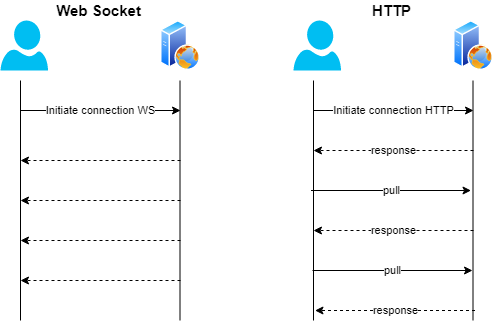
\includegraphics[width=0.7\textwidth]{images/websocket-vs-http.png}
    \caption{WebSocket vs HTTP: Persistent vs Short-Lived Connections}
    \label{fig:websocket-vs-http}
\end{figure}

In addition to its efficiency, the WebSocket protocol supports bi-directional communication, allowing both the client and server to send messages independently at any time. This is a major improvement over HTTP, where the client must always initiate communication. The protocol operates over a single TCP connection, which simplifies firewall traversal and network management. Security is addressed through the use of the wss:// scheme, which encrypts WebSocket traffic using TLS. As a result, WebSocket has become the protocol of choice for building interactive, real-time web applications that demand high responsiveness and scalability.

\subsection{Redis / Message Brokers}
Redis is a popular choice for message brokering and caching in real-time systems due to its high performance and support for pub/sub patterns \cite{redisdocs,nguyen2021pubsub,blogkafka2022}. Distributed message brokers such as Kafka are also increasingly used to support large-scale, fault-tolerant deployments \cite{blogkafka2022,gonzalez2022websocket}.

\subsection{Load Balancing and Reverse Proxies}

Load balancing and reverse proxy solutions are essential components in modern web architectures, especially for real-time messaging systems. A reverse proxy acts as an intermediary between clients and backend servers, receiving requests from the internet and forwarding them to the appropriate server. This setup not only helps distribute incoming traffic evenly across multiple servers but also enhances security by hiding the internal server structure from external users. Load balancers can detect server health and automatically reroute traffic if a server becomes unavailable, ensuring high availability and reliability. By managing connection surges and distributing workloads, these solutions prevent individual servers from becoming overwhelmed during peak usage.

\begin{figure}[H]
    \centering
    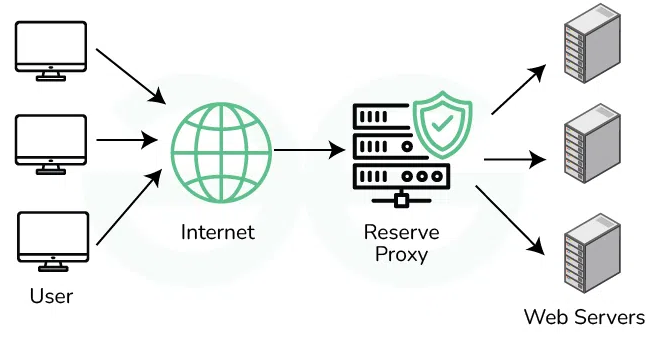
\includegraphics[width=0.7\textwidth]{images/Reverse-Proxy.png}
    \caption{Reverse Proxy: Handling Internet Requests for Multiple Servers}
    \label{fig:reverse-proxy}
\end{figure}

In addition to balancing loads, reverse proxies often provide features such as SSL termination, caching, and compression, which further optimize performance and security. They can also enforce access controls and monitor traffic for malicious activity, acting as a first line of defense against attacks. Popular tools like Nginx and HAProxy are widely used due to their robustness and configurability. In real-time systems, reverse proxies play a crucial role in maintaining low latency and seamless user experiences by efficiently routing requests and managing persistent connections. Their ability to scale horizontally by adding more backend servers makes them indispensable for large-scale, distributed applications.

\subsection{Real-Time Frameworks / Libraries}
A variety of frameworks and libraries have emerged to simplify the development of real-time features, including Socket.IO, uWebSockets.js, and SignalR \cite{tilkov2018nodejs,rauch2022scalable,blogmicro2023}. These tools abstract away protocol details and provide robust APIs for developers.

\section{Theoretical Principles and Architectural Models}
The design of scalable messaging systems is grounded in theoretical principles such as event-driven architecture, publish–subscribe models, and microservices \cite{fowler2015microservices,kleppmann2013designing,nguyen2021pubsub}. These models enable modularity, extensibility, and efficient resource utilization \cite{guth2018comparison,li2020realtime}.

\subsection{Event-Driven Architecture}
Event-driven architecture allows systems to react to changes and user actions in real time, supporting high concurrency and responsiveness \cite{tilkov2018nodejs,smith2020cloud}. This paradigm is widely adopted in Node.js-based messaging platforms \cite{cantelon2017nodejs,blogmicro2023}.

\subsection{Publish–Subscribe Model}
The publish–subscribe model decouples message producers from consumers, enabling scalable fan-out and flexible communication patterns \cite{nguyen2021pubsub,redisdocs,blogkafka2022}. This approach is fundamental to the architecture of modern real-time messaging systems \cite{gonzalez2022websocket,kim2023iot}.

\subsection{Microservices vs Monolithic Approaches}
Microservices architectures offer improved scalability, maintainability, and fault isolation compared to monolithic designs \cite{fowler2015microservices,smith2020cloud,blogmicro2023}. However, they also introduce challenges in service coordination and distributed state management \cite{kleppmann2013designing,li2020realtime}.

\subsection{Horizontal Scaling Principles}
Horizontal scaling enables systems to handle increased load by adding more nodes, rather than upgrading individual servers \cite{zhang2021aws,kim2023iot}. This principle is essential for supporting large numbers of concurrent users in real-time messaging applications \cite{guth2018comparison,wang2018scalable}.

\subsection{Consistency Models in Messaging Systems}
Consistency models define how updates are propagated and observed in distributed messaging systems \cite{kleppmann2013designing,li2020realtime,nguyen2021pubsub}. The choice of consistency model impacts system performance, user experience, and fault tolerance \cite{guth2018comparison,blogkafka2022}.

\section{Summary}
This chapter has reviewed existing real-time messaging solutions, relevant technologies, and theoretical principles that underpin the design of scalable messaging systems. The insights gained from this literature review will inform the design and implementation choices made in subsequent chapters.

\lipsum[14]
